\documentclass[accentcolor=tud1b,colorbacktitle,landscape,german,presentation]{tudbeamer}

%Includes
\usepackage{float}
\usepackage{listings}
\usepackage{color}
\usepackage{graphicx}
\usepackage{epstopdf}
\usepackage{wrapfig}
%Deutsche Silbentrennung
\usepackage[ngerman]{babel}
%Deutsche Umlaute
\usepackage[utf8]{inputenc}
\usepackage{adjustbox}
\usepackage{hyperref}
\usepackage{pdfpcnotes}

\setbeamerfont{note page}{size=\large}

\DeclareGraphicsExtensions{.pdf,.png,.jpg}
\graphicspath{ {./img/} }

\title[]{Entwicklung eines zentralen \\Steuerungsprogramms für einen \\Forschungsflugsimulator}
\subtitle{{\scriptsize Vortragender: Tim Weißmantel 
	\\Team: Frederik Bark, Heiko Carrasco, Jonas Meurer und Leonardo Zaninelli}}
\institute{BP WS 2017/18 | Entwicklung eines zentralen Steuerungsprogramms für einen Forschungsflugsimulator}
\date{\today}

\newcommand{\ftitle}{

	\frametitle{\insertsectionhead \\ {\small \insertsubsectionhead}}
}

\begin{document}

%Deckblatt
\begin{titleframe}
	\begin{figure}
		\centering
		\includegraphics[scale=0.21]{simulator_3_intro}
	\end{figure}
	\pnote{Willkommen}
	\pnote{Gruppe 19}
\end{titleframe}

\section{Kontext}
\subsection{der Flugsimulator}
\begin{frame}
	\ftitle
	\begin{figure}
		\centering
		\includegraphics[scale=0.055]{simulator_4}
	\end{figure}

	\pnote{Auftraggeber Institut für Flugsysteme und Regelungstechnik}
	\pnote{an der Lichtwiese}
	\pnote{wird zum Forschen im Bereich Führungsysteme (Flugverkehr) verwendet}
\end{frame}

\subsection{das Problem}
\begin{frame}
	\ftitle
	\begin{figure}
		\centering
		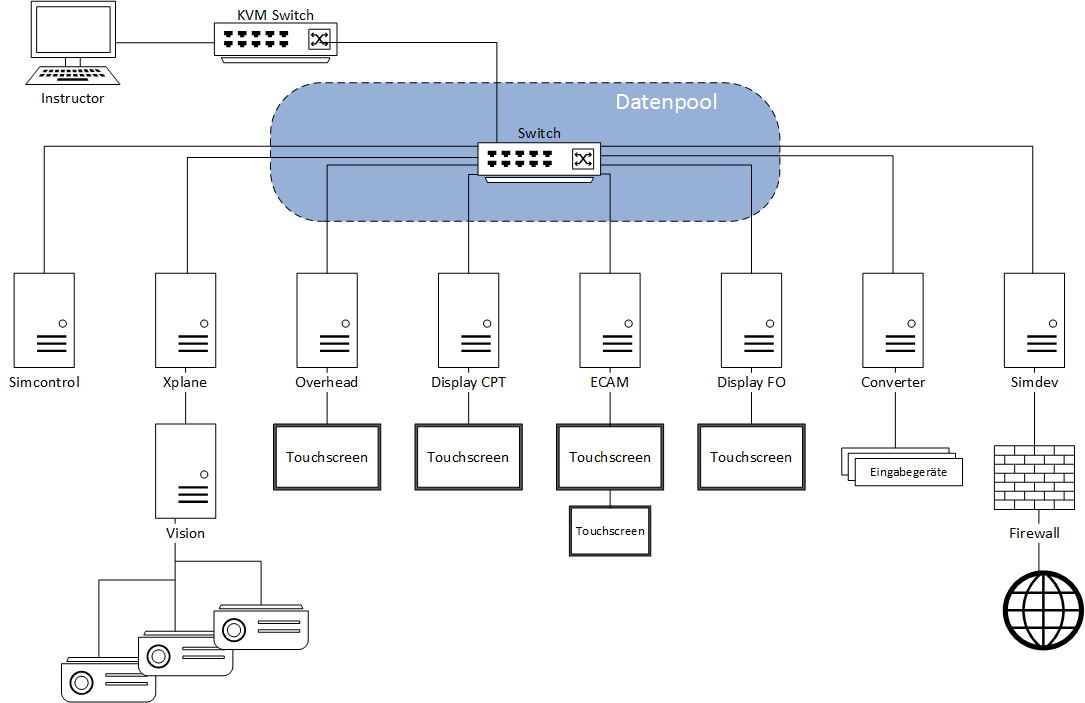
\includegraphics[scale=0.23]{aufbau}
		\includegraphics[scale=0.035]{server}
	\end{figure}
	
	\pnote{komplexes System}
	\pnote{entstanden über einen zeitraum von ca 15 Jahren}
	\pnote{wurde oft erweitert}
	\pnote{viel unterschiedliche Hardware}
	\pnote{jedes Programm muss per Hand gestartet werden}
	\pnote{Autostart nicht möglich, wegen Datenpool und unterschiedlichen Szenarien}
	\pnote{geübte Personen ca 10 Minuten}
	\pnote{ungeübte Personen ca 30 Minuten oder sogar mehr}
\end{frame}

\section{Software}
\subsection{}
\begin{frame}
	\ftitle
	Features:
	\begin{itemize}
		\item starten/steuern eines einzelnen Clients über eine Benutzeroberfläche
		\item erstellen und ausführen von Scripts zur Automatisierung des Startvorgangs
	\end{itemize}
	\vspace{0.5cm}
	Sprache:
	\begin{figure}
		\centering
		
\includegraphics[scale=0.05]{python}
	\end{figure}
\end{frame}

\subsection{Aufbau}
\begin{frame}
	\ftitle
	\begin{figure}
		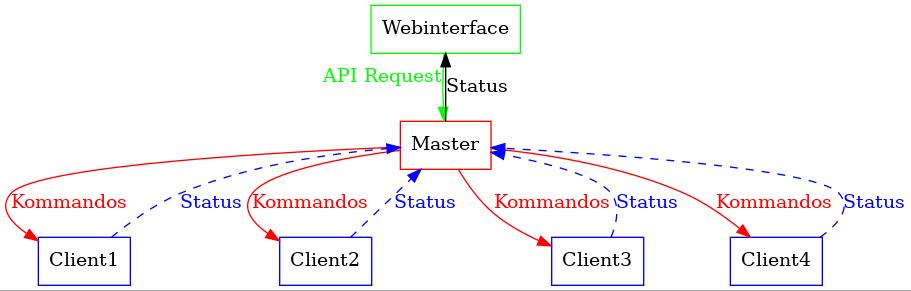
\includegraphics[scale=0.35]{master-client}
	\end{figure}
	\pnote{Interface als Website}
	\pnote{Kommunikation über Websockets}
\end{frame}


\subsection{Fortschritt}
\begin{frame}
	\ftitle
	\begin{figure}
		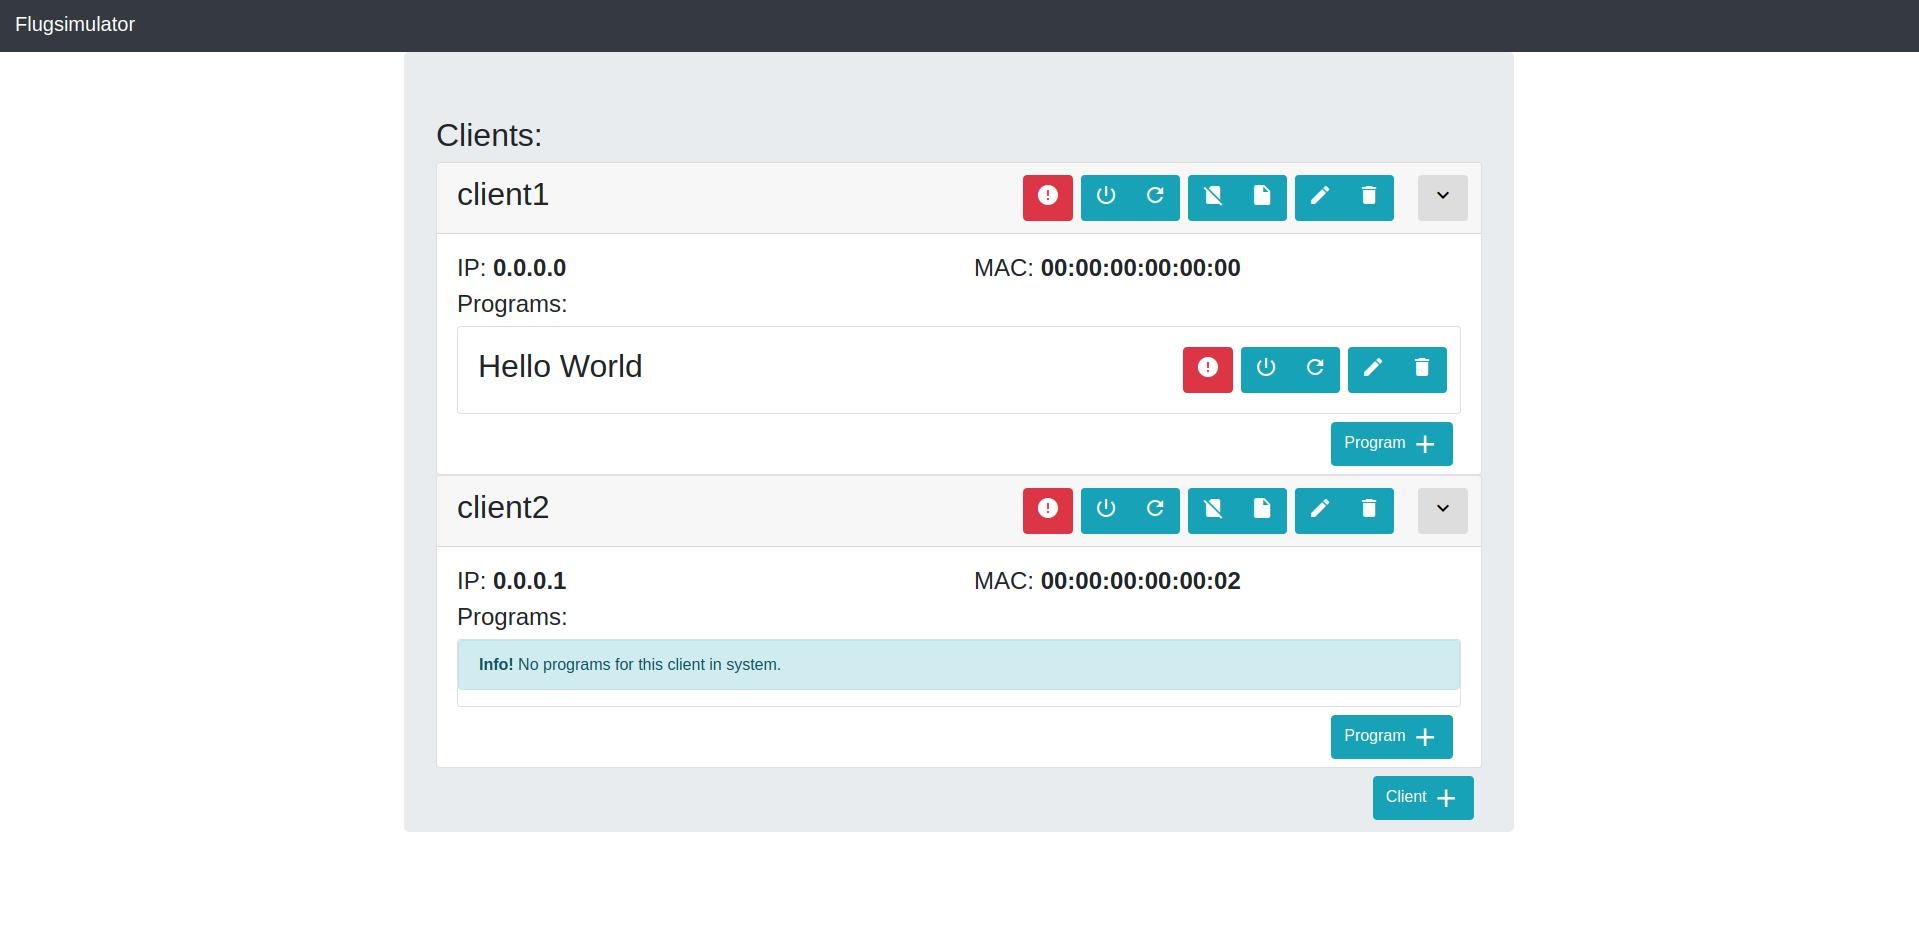
\includegraphics[scale=0.18]{screenshoot}
	\end{figure}
	
	\pnote{hinzufügen von Clients im Webinterface}
	\pnote{hinzufügen von Programmen auf Clients im Webinterface}
	\pnote{wake on Lan}
	\pnote{grobe Implementierung von Master/Slave system}
\end{frame}

\section{Qualitätssicherung}
\subsection{Portabilität}
\begin{frame}
	\ftitle
	Die Software für die Clients muss auf vielen verschiedenen Systemen laufen:\\[5pt]
	\begin{enumerate}
		\item Hohe Testabdeckung (mindestens 90\%):
		\begin{itemize}
			\item 
\includegraphics[scale=0.1]{coveralls}
		\end{itemize}
		\item Viele Testumgebungen:
		\begin{itemize}
			\item 
\includegraphics[scale=0.1]{travisci} \hspace*{2cm} (Linux)
			\item 
\includegraphics[scale=0.1]{appveyor} \hspace*{1.55cm} (modernes Windows)
			\item 
\includegraphics[scale=0.1]{jenkins} \hspace*{2.5cm} (Windows XP)
		\end{itemize}
	\end{enumerate}

	\pnote{Software für Master wird auf modernem System laufen}
\end{frame}

\begin{frame}
	\ftitle	
	Zusammengefasst in Pullrequests von Github für jede Userstory:\\
	\begin{figure}
		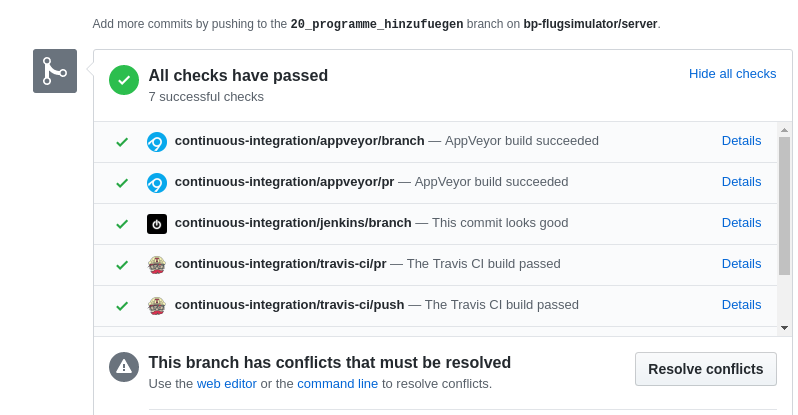
\includegraphics[scale=0.3]{github_integration}
	\end{figure}

	\pnote{für jede Userstory wird ein Pullrequests auf Github gemacht}
	\pnote{dient auch als Forum für Implementierungen}
\end{frame}

\begin{frame}
	\ftitle
	Vor dem mergen einer Userstory wird eine Liste abgearbeitet:
	\begin{figure}
		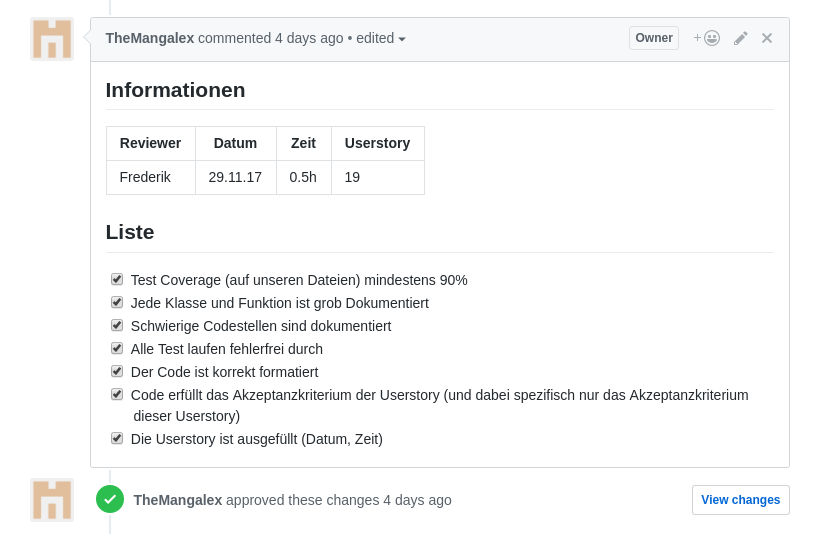
\includegraphics[scale=0.29]{github_list}
	\end{figure}
	\pnote{falls eine Punkt nicht erfüllt wird, muss der Entwickler der Userstory 
		das Problem beheben}
\end{frame}

\subsection{Benutzbarkeit}
\begin{frame}
	\ftitle
	Auch andere Personen am Institut müssen das Interface verwenden können.
	\begin{enumerate}
		\item Nutzerstudie
		\item Benutzeranleitung
	\end{enumerate}
\end{frame}

\section{Zeiterfassung}
\begin{frame}
	\ftitle
	Userstorys der ersten Iteration:
	\begin{figure}
		\begin{tabular}{|c|l|c|c|}
			\hline
			ID&Namen&Storypoints&Stunden \\ \hline \hline
			1 &Willkommensnachricht&10&2 \\ \hline
			16&Slaves anzeigen&4&4\\ \hline
			2 &Slaves registrieren&8&30\\ \hline
			16&Kontextmenü&10&10\\ \hline
			14&Slaves löschen&4&9\\ \hline
			15&Slaves bearbeiten&4&3\\ \hline
		\end{tabular}
	\end{figure}

	\pnote{Willkommensnachricht wurde stark überschätzt}
	\pnote{für Slaves registrieren gab es 3 verschiedenen Ansätze die viel Diskutiert wurden}
	\pnote{in Slaves löschen und Slaves registrieren wurde viel Vorarbeit für Slaves bearbeiten  gemacht}
\end{frame}

\section{}
\begin{frame}
	\begin{center}
		\textbf{\LARGE{Fragen?}}
	\end{center}
\end{frame}
\end{document}